\fancyhead{}
\fancyfoot{}
\newtheorem{teorema}{Teorema}
\cfoot{\thepage}
\setlength{\headheight}{15pt}  % O 14.5pt, según la sugerencia



\lhead{Conceptos fundamentales, teorías y antecedentes}
%\rhead{\today}
%\rfoot{\thepage}

\chapter{Conceptos fundamentales, teorías y antecedentes}


\section{Conceptos fundamentales}
\subsection{Toma de decisiones}
La toma de decisiones es el proceso de seleccionar una acción entre varias alternativas, siguiendo una serie de etapas clave: \\
Identificación del problema: Definir claramente la situación que requiere una decisión.\\
Recopilación de información: Obtener datos relevantes sobre el problema y las posibles soluciones.\\
Análisis de alternativas: Evaluar ventajas y desventajas de cada alternativa.\\
Selección de la mejor alternativa: Elegir la opción que mejor cumpla los criterios establecidos.\\
Implementación y seguimiento: Aplicar la decisión y monitorear su efectividad.\\
Durante todo el proceso, se deben considerar factores como el impacto económico, el tiempo de implementación, el riesgo de resultados no deseados y los beneficios en relación con los objetivos organizacionales.\\
\subsection{Sistema Experto}
Definición \\
Un sistema experto (SE) es un sistema de inteligencia artificial diseñado para emular el conocimiento y la experiencia de un experto humano en un dominio específico \cite{Leo}.
Componentes principales \\
Base de conocimiento: Almacena hechos, reglas y relaciones sobre el dominio del problema.\\
Motor de inferencia: Aplica reglas para razonar y llegar a conclusiones.\\
Interfaz de usuario: Permite la interacción entre el usuario y el sistema experto.\\
Clasificación de los SE \\
Basados en reglas o enfoque simbólico \\
Utilizan reglas explícitas escritas por expertos.\\
No aprenden automáticamente, sino que dependen de la base de conocimientos creada manualmente.
Ejemplo: Sistemas de diagnóstico médico que aplican reglas "Si X, entonces Y" \cite{Raul}.\\

Basados en casos o machine learning (aprendizaje basado en casos)\\
Guardan experiencias pasadas y las comparan con nuevos problemas para hacer predicciones o recomendaciones.
Se relacionan con enfoques de aprendizaje supervisado o técnicas como k-Nearest Neighbors (k-NN).\\
Ejemplo: Un sistema que recomienda soluciones basándose en casos previos de fallos en una máquina.
Basados en modelos: Enfoque estadístico y también Machine Learning en algunos casos
utilizan modelos matemáticos o estadísticos para tomar decisiones.\\
Pueden incluir técnicas de aprendizaje automático como redes neuronales o regresión logística.\\
Ejemplo: Un sistema que predice fallos en un equipo usando modelos probabilísticos o redes neuronales.\\
\\
Características de los SE\\
Especialización en un dominio específico.\\
Uso de reglas predefinidas para la toma de decisiones.\\
Capacidad de explicar el razonamiento detrás de sus conclusiones.\\
Posibilidad de aprendizaje y adaptación a nuevas experiencias\cite{Raul}.\\


\begin{figure}[H]
  \begin{center}
  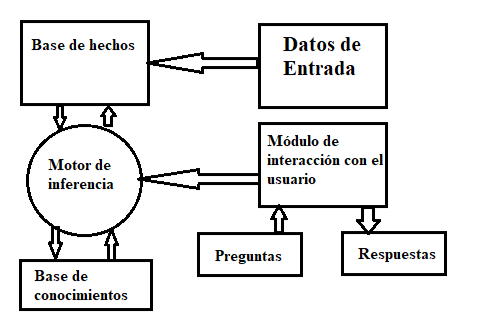
\includegraphics[scale = 1.0]{./images/grafico}
  \caption{Arquitectura del sistema experto.}
  \label{fig:grafico}
  \end{center}
  \end{figure}
  \subsection{Monitoreo de Sistemas}
  Definición
  El monitoreo de sistemas consiste en recopilar y analizar datos de un sistema para detectar anomalías y posibles fallas, con el objetivo de optimizar su funcionamiento y prevenir problemas antes de que ocurran.\\
  Técnicas de Monitoreo\\
  Recolección de datos: Mediante sensores o software de monitoreo.\\
  Análisis de datos: Identificación de tendencias y patrones.\\
  Interpretación de datos: Comprensión del significado de las variaciones en los datos.\\
  Generación de alertas: Notificación de anomalías a través de alertas visuales o sonoras.\\
  Un componente clave en este proceso es el módulo de adquisición de datos, que recoge y procesa información proveniente de diversos dispositivos dentro de un sistema.\\
  \subsection{Fábrica de PVC}
  Policloruro de Vinilo (PVC)
  El PVC es un polímero termoplástico utilizado en diversas aplicaciones industriales por su durabilidad y versatilidad. Su procesamiento industrial requiere un control preciso de temperatura para garantizar la calidad del producto final. \cite{Luis}\\
  Métodos de Fabricación\\
  Extrusión: El PVC fundido pasa a través de una matriz para formar productos largos y uniformes.\\
  Moldeo por inyección: El PVC fundido se inyecta en un molde para fabricar objetos detallados.\\
  Calandrado: El PVC se lamina en delgadas hojas al pasar por una serie de rodillos.\\
  Moldeo por soplado: Similar al moldeo por inyección, pero con un paso adicional para formar objetos huecos.\\
  En todos estos procesos, el refrigerante principal es el agua.\\

  \subsection{Criterios y Condiciones para los Sistemas de Refrigeración Industrial.}
  El enfriamiento del PVC es una fase crítica en la producción industrial, ya que afecta:\\
  Calidad del producto: Un enfriamiento adecuado evita defectos y tensiones internas.\\
  Eficiencia del proceso: Un sistema de refrigeración eficiente reduce costos operativos y tiempos de producción, es un
  parámetros clave en la refrigeración del PVC.\\
  Control de temperatura: Evitar fluctuaciones bruscas que puedan afectar la calidad.\\
  Velocidad de enfriamiento: Debe ser gradual para evitar deformaciones.\\
  Distribución uniforme del flujo de agua: Para prevenir puntos calientes o fríos en el material.\\
  \subsection{Fallas Comunes en Sistemas de Refrigeración Industrial}
  Los sistemas de refrigeración industrial pueden presentar diversas fallas que afectan su rendimiento \cite{Zamo}.\\
  Compresor sobrecargado: Puede deberse a un dimensionamiento incorrecto, falta de lubricación o fallas eléctricas.\\
  Pérdida de refrigerante: Ocasionada por fugas en juntas, válvulas o tuberías defectuosas.\\
  Problemas de circulación de agua: Puede ocurrir por bloqueos en tuberías o fallas en la bomba de circulación.\\
  Condensador sucio u obstruido: La acumulación de suciedad reduce la eficiencia del intercambio de calor.\\
  Problemas en el evaporador: Puede bloquearse por acumulación de suciedad o escarcha en las bobinas.\\
  Fallas en el sistema de control: Sensores defectuosos o controladores dañados pueden generar lecturas incorrectas.\\
  Problemas de presión: Fluctuaciones anormales pueden deberse a fugas de refrigerante o insuficiente flujo de agua.\\
  Corrosión y erosión: Factores como la calidad del agua y la velocidad del flujo pueden deteriorar los componentes.\\
  Un adecuado monitoreo y mantenimiento preventivo son esenciales para minimizar estas fallas y garantizar la operatividad del sistema.\\
  
\section{Antecedentes}
\subsection{Antecedente 1}
Diseño de sistema de control automatizado y utilización de software para
la monitorización remota de equipos de refrigeración industrial de bajo costo,
en la industria de conservación de medicamentos \cite{Nava}.\\ \\
Título: Diseño de sistema de control automatizado y utilización de software para la monitorización remota de equipos de refrigeración industrial de bajo costo, en la industria de conservación de medicamentos.\\
Autores: Navarrete Enderica, Víctor Alejandro \\
Año: 28-feb-2020 \\
Problemática: \\
Los equipos de refrigeración en la industria farmacéutica presentan limitaciones en su funcionamiento, lo que compromete la calidad y conservación de los productos farmacéuticos. La falta de monitoreo adecuado puede generar fallas en los equipos, incrementando rápidamente la temperatura interna de los cuartos de almacenamiento y afectando negativamente la calidad de los medicamentos.\\
Objetivo General \\
Desarrollar un sistema de control automatizado y supervisión remota para equipos de refrigeración industrial, permitiendo evaluar los estados y procesos de manera eficiente mediante la utilización de equipos de bajo costo. Este sistema tiene como objetivo optimizar el control de temperatura en cuartos refrigerados y asegurar la calidad de los productos farmacéuticos.\\
Metodología \\
Se utiliza una metodología de tipo correlacional con un enfoque cuantitativo. Se realiza una evaluación mediante simulaciones y pruebas con equipos reales en un entorno de trabajo real. El sistema propuesto es evaluado en términos de su desempeño en situaciones de fallo para comprobar su efectividad en la mejora del control de temperatura.\\
Herramientas (¿Qué instrumentos utilizó?)\\
Software de simulación para evaluar los procesos de control.
Equipos de control y supervisión de bajo costo (PLC, válvulas de expansión electrónicas, etc.).
Técnicas de automatización y supervisión remota.
Resultados más importantes \\
Se obtiene un sistema supervisorio y de control que mejora la eficiencia y optimización del control de temperatura en cuartos refrigerados.
El sistema demuestra su funcionalidad mediante simulaciones y pruebas con equipos reales.
Se garantiza la mejora en el control de los equipos de refrigeración industrial y en la conservación de medicamentos.\\
Similitud y diferencia con el TFG \\
Similitudes: Ambos trabajos se centran en la implementación de sistemas de monitoreo y control automatizado para equipos industriales críticos (refrigeración).\\
Se hace uso de la inteligencia artificial o software de control para optimizar los procesos de monitoreo en tiempo real.\\
Ambos se enfocan en la mejora de la eficiencia y la fiabilidad de los sistemas, así como en la prevención de fallas que puedan comprometer la seguridad o calidad de los productos.\\
Diferencias: El trabajo propuesto se enfoca en la industria farmacéutica y el control de la conservación de medicamentos, mientras que mi TFG está más orientado hacia la producción de plásticos.\\
Mi trabajo utiliza un sistema experto basado en reglas para la detección de fallas en las máquinas críticas, mientras que el trabajo de Navarrete se enfoca en un sistema automatizado de control y supervisión utilizando PLC y equipos de control de bajo costo.\\
Fuente: Universidad Católica de Santiago de Guayaquil Navarrete Enderica, Víctor Alejandro 28-feb-2020


\subsection{Antecedente 2}
Automatización de sistema de refrigeración de un edificio (chiller 270 tons)
con sistema de alarma vía GSM y encendido automático en caso de elevación
de temperatura en centro de cómputo \cite{Lema}. \\

Título: Automatización del sistema de refrigeración con control de temperatura y sistema de alarma GSM en un edificio de oficinas \\
Autor: Oscar Leonardo Reyes Lema \\
Año: 2016 \\
Problemática: \\
Los sistemas de refrigeración en un edificio de oficinas presentan problemas de eficiencia y consumo energético, lo que puede generar fallas en el funcionamiento del centro de cómputo. Además, la falta de monitoreo adecuado y respuesta rápida ante fallas provoca ineficiencia operativa y posibles daños en los equipos.\\
Objetivo General: \\
Diseñar y automatizar un sistema de refrigeración que permita mantener el control de la temperatura en un edificio de oficinas, asegurando su correcto funcionamiento y reduciendo el consumo energético.
Metodología: \\
Se implementó un sistema basado en PLC Siemens y microcontroladores PIC para monitorear y controlar la temperatura. Además, se incluyó un sistema de alarma GSM para notificar fallas a los supervisores mediante mensajes de texto. Se realizaron pruebas de validación para comprobar la eficacia del sistema.\\
Herramientas: \\
PLC Siemens
Microcontroladores PIC
Sensores de temperatura
Sistema de alarma GSM
Software de control y monitoreo
Resultados más importantes: \\
Se logró reducir el consumo energético del sistema de refrigeración del 55 al 30 por ciento.\\
El sistema de alarma GSM permitió una respuesta más rápida ante fallas.\\
Se optimizó el control de temperatura, asegurando condiciones adecuadas para el centro de cómputo.\\

Similitud y diferencia con el TFG\\
Similitudes:\\
Ambos proyectos buscan mejorar la eficiencia de sistemas de refrigeración a través de la automatización y monitoreo en tiempo real. \\
Prevención de fallas: Tanto el sistema del edificio como el de la producción de plásticos se enfocan en detectar y anticipar posibles fallos para evitar pérdidas económicas y tiempos de inactividad. \\
Uso de sensores y sistemas de control: Ambos estudios emplean sensores de temperatura para la regulación de los equipos. \\
Optimización operativa: Los dos proyectos buscan automatizar procesos para mejorar la sostenibilidad y la eficiencia energética. \\
Diferencias: \\
Ámbito de aplicación: El trabajo de automatización se enfoca en un edificio de oficinas y centro de cómputo, mientras que mi investigación se centra en la producción de plásticos. \\
Tecnología utilizada: En el otro trabajo se usan PLC Siemens y microcontroladores PIC, mientras que en mi investigación se utilizan un sistema experto basado en reglas con inteligencia artificial y software open source. \\
Enfoque en la calidad del producto: Tu TFG está orientado a evitar variaciones de temperatura que afectan la calidad del plástico, mientras que el otro estudio se enfoca en garantizar condiciones óptimas en un centro de cómputo. \\
Mecanismo de alerta: El sistema del otro trabajo utiliza alarma GSM para notificaciones a los supervisores, mientras que en mi sistema se implementa un sistema experto que gestiona las alarmas y toma decisiones en tiempo real. \\

\subsection{Antecedente 3}
Sistema de detección y diagnóstico de fallas de un proceso térmico mediante
inteligencia artificial \cite{Var} . \\
Título:\\
Sistema de Detección y Diagnóstico de Fallas de un Proceso Térmico mediante Inteligencia Artificial. \\
Autores: \\
Rincón Aristizábal, L. F., \& Vargas Chavarro, D. A. (2018). \\
Problemática: \\
El trabajo aborda la problemática relacionada con la detección y diagnóstico de fallas en un proceso térmico utilizado en sistemas industriales. Se centra en la dificultad de mantener la eficiencia de los procesos industriales debido a fallas imprevistas, lo cual puede causar pérdidas económicas y riesgos operativos. La solución se orienta a la detección temprana de estos fallos para mejorar la seguridad y eficiencia del proceso.\\
Objetivo General: \\
Desarrollar un sistema para la detección y diagnóstico de fallas en un proceso térmico utilizando Inteligencia Artificial, mediante el uso de Redes Neuronales Artificiales (RNA) para procesar datos provenientes de los sensores y emitir alertas sobre posibles fallas.\\
Metodología: \\
Se utilizó un enfoque basado en Inteligencia Artificial, más específicamente, una Red Neuronal Artificial (RNA). Los datos de sensores de temperatura y caudal se recopilaron mediante una tarjeta de adquisición de datos y fueron procesados utilizando herramientas como LabView y MatLab. Luego, se diseñó una interfaz gráfica de usuario (GUI) para mostrar el diagnóstico de fallas.\\
Herramientas (¿Qué instrumentos utilizó?): \\
LabView: Para la adquisición y exportación de los datos a Excel. \\
MatLab: Para el diseño de la interfaz gráfica y la implementación de la Red Neuronal Artificial (RNA). \\
Tarjeta de adquisición de datos EDIBON: Para obtener señales de los sensores de temperatura y caudal del proceso térmico. \\
Resultados más importantes: \\
Se obtuvo una interfaz gráfica de usuario (GUI) que proporciona al operador de la planta un diagnóstico claro sobre la ubicación de las fallas dentro del sistema térmico.\\
El sistema es capaz de comparar los datos actuales de los sensores con un modelo de operación normal y detectar fallas en dispositivos como el tanque de proceso, enfriador o intercambiador.\\
El sistema permite la detección de fallas como desconexión de sensores, problemas con la tarjeta de adquisición de datos o daños eléctricos en la fuente.\\
Similitudes: \\
Uso de Inteligencia Artificial para diagnóstico de fallas: \\
Ambos trabajos utilizan tecnologías de Inteligencia Artificial para diagnosticar fallas en sistemas industriales. En mi caso, se emplea un sistema experto basado en reglas, mientras que el trabajo de referencia usa Redes Neuronales Artificiales.\\
Monitoreo en tiempo real: \\
Los dos proyectos incluyen monitoreo en tiempo real de los equipos críticos. En mi caso, se monitorean los sistemas de refrigeración de agua en la producción de plásticos, y en el caso del trabajo de referencia, se monitorea un proceso térmico industrial.\\
Optimización del mantenimiento y prevención de fallas: \\
Ambos trabajos tienen como objetivo mejorar la eficiencia operativa y prevenir fallas imprevistas en los sistemas. La detección temprana de fallas es clave para reducir tiempos de inactividad no planificados y evitar pérdidas económicas.\\
Aplicación en la industria: \\
Ambos trabajos abordan el uso de estas tecnologías en un contexto industrial para mejorar la seguridad y eficiencia de los procesos de producción.\\

Diferencias: \\
Tecnología de Inteligencia Artificial utilizada: \\
El trabajo de referencia emplea Redes Neuronales Artificiales (RNA), mientras que, en mi investigación, el sistema experto se basa en reglas predefinidas para el diagnóstico de fallas.\\
Tipo de procesos monitoreados: \\
Mi trabajo se centra en el monitoreo de equipos de refrigeración de agua en la producción de plásticos, mientras que el trabajo de referencia está relacionado con el monitoreo de procesos térmicos en sistemas industriales.\\
Herramientas utilizadas: \\
El trabajo de referencia utiliza LabView y MatLab para la recopilación de datos y diseño de la interfaz gráfica, mientras que en mi investigación se utiliza software open source. \\
Enfoque de diagnóstico: \\
Mientras que el trabajo de referencia se enfoca en la detección de fallas dentro de un proceso térmico específico, mi investigación aborda el monitoreo de equipos de refrigeración, un sistema con distintos parámetros críticos como temperatura, caudal, bomba de agua, etc. \\
Fuente: \\
Rincón Aristizábal, L. F., Vargas Chavarro, D. A. (2018). Sistema de Detección y Diagnóstico de Fallas de un Proceso Térmico mediante Inteligencia Artificial. Trabajo de grado, Universidad Distrital Francisco José de Caldas, Facultad Tecnológica, Programa de Ingeniería Mecánica, Bogotá. \\


